% !TeX encoding =UTF-8
% !TeX spellcheck =it_IT
% !TeX root =MatDiz.tex
\chapter{R}
\vspace{5mm} 
\lemma{radice}
\lemma{radiante}\pointsto~\vedilemma{a. misura}
\lemma{reciproco}
\lemma{Recorde Robert} (1510-1558)\index{Recorde Robert} Scrisse il primo trattato inglese di algebra \foreignlanguage{english}{\textit{The Whetstone of Witte}}  dove venne usato per la prima volta il simbolo $=$ nel  1557\cite{Kline1972}.
\begin{figure}
\centering\scaptionb{Robert Recorde (1510-1558)}
	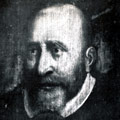
\includegraphics[width=0.7\linewidth]{Figure/R/Robert_recorde}
	\label{fig:robertrecorde}
\end{figure}
\lemma{Rhind Henry}Alexander Henry (1833–1863) Scozzese, archeologo trovò in un mercato di Luxor nel 1858, il papiro che porta il suo nome\index{Rhind Henry}. 
\lemma{raggio}Segmento che ha per estremi il centro di una circonferenza\pointsto~\vedilemma{circonferenza} e un punto di questa. 
\begin{figure}
	\centering\scaptionb{Alexander Henry Rhind (1833–1863)}
	\label{fig:frontispiecetomemoirofthelatealexanderhenryrhindofsibster}
	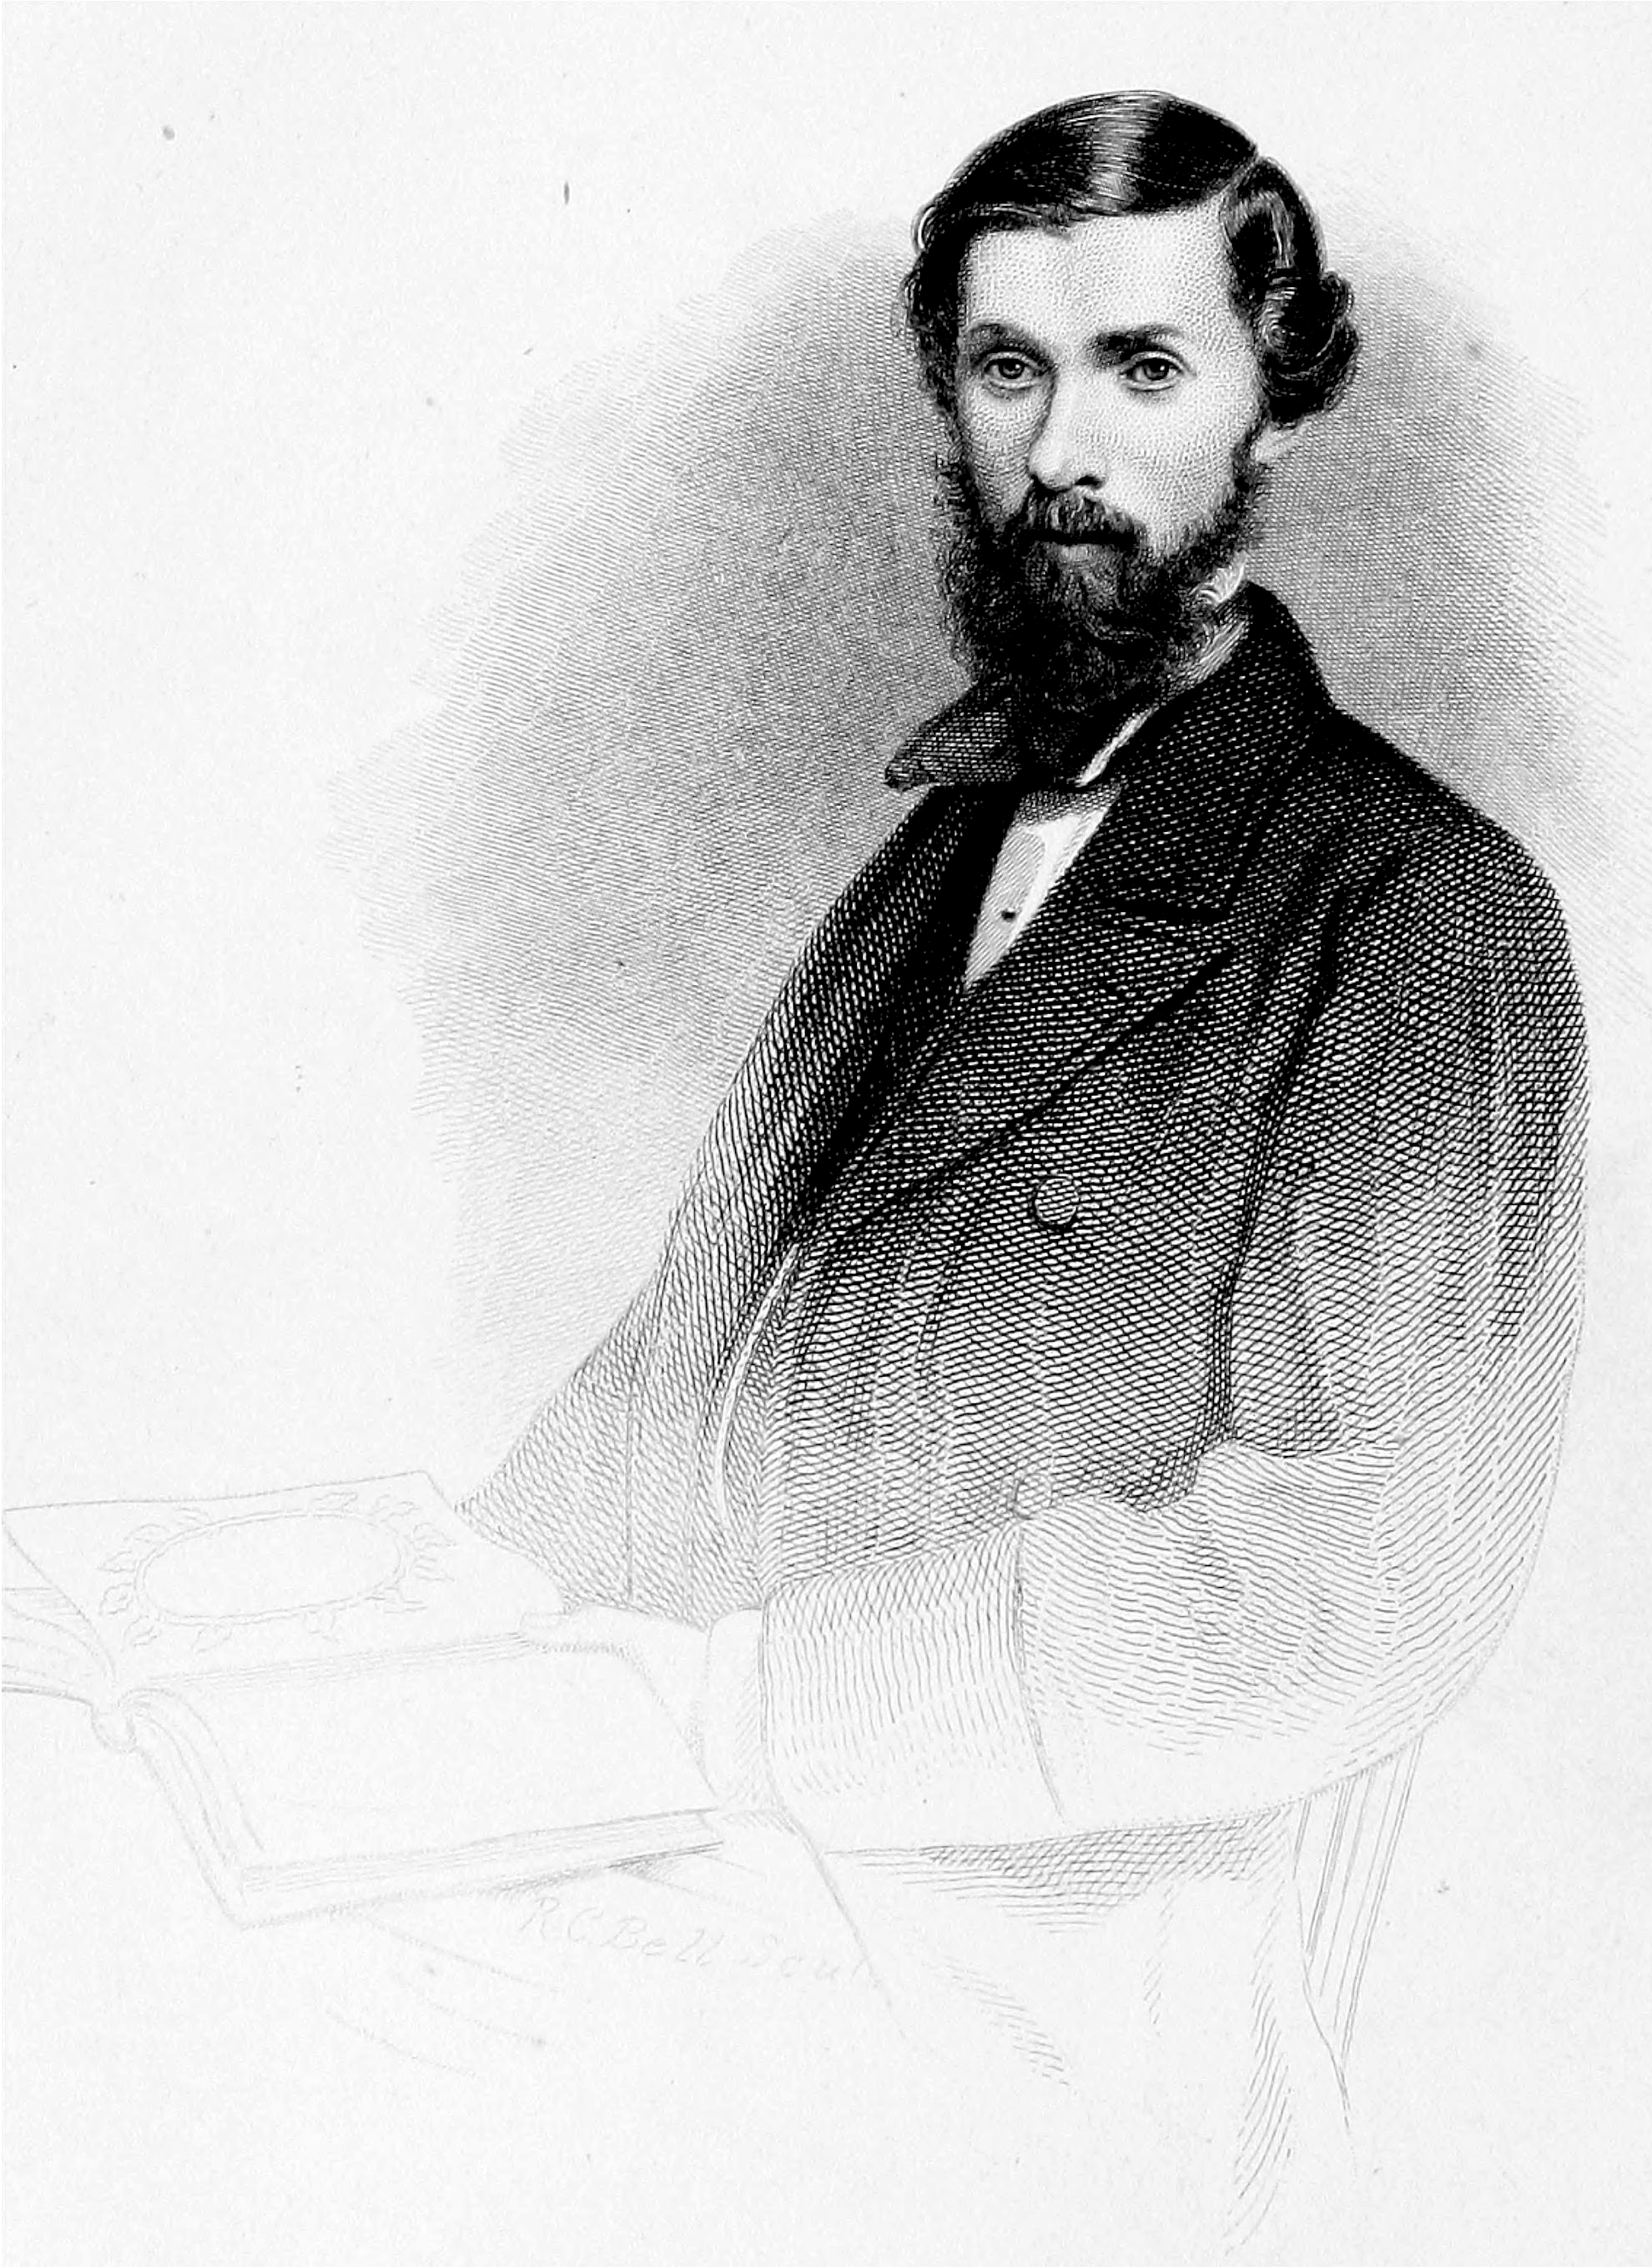
\includegraphics[width=0.7\linewidth]{Figure/R/Frontispiece_to_Memoir_of_the_late_Alexander_Henry_Rhind,_of_Sibster}
\end{figure}
\lemma{relazione}
\lemma{retta}Per Euclide\pointsto~\seeentry{Euclide}\index{Euclide} ente geometrico fondamentale insieme a punto e piano.
\llemma{r. complanari}Rette che appartengono allo stesso piano.
\llemma{r. incidenti}Rette complanari che hanno un punto in comune.
\llemma{r. parallele}Rette complanari che non hanno un punto in comune.
\llemma{r. perpendicolari}
Se due rette sono incidenti e formano quattro angoli retti le rette sono perpendicolari.
\llemma{r. sghembe}Rette non complanari che non hanno punti in comune.